\documentclass[10pt,letterpaper]{article}
\usepackage[margin=0.68in,top=0.72in,bottom=0.72in]{geometry}
\usepackage[T1]{fontenc}
\usepackage[scaled=0.96]{helvet}
\renewcommand{\familydefault}{\sfdefault}
\usepackage{amsmath,amssymb,array,booktabs,tabularx,tikz,fancyhdr,enumitem}
\usepackage[hidelinks]{hyperref}
\usetikzlibrary{arrows.meta}
\setlength{\parindent}{0pt}
\setlength{\parskip}{6pt}
\setlist[itemize]{leftmargin=15pt,itemsep=3pt,topsep=3pt}
\setlist[enumerate]{leftmargin=18pt,itemsep=3pt,topsep=3pt}
\pagestyle{fancy}\fancyhf{}
\fancyhead[L]{\small Week 62 / Conflict networks / Adult guide}
\fancyfoot[L]{\small Bellingham Math Circle / Week 62 / W62-FAC-v1}
\fancyfoot[R]{\small\thepage}
\renewcommand{\headrulewidth}{0.3pt}\renewcommand{\footrulewidth}{0pt}
\setlength{\headheight}{14pt}
\setlength{\headsep}{15pt}
\setlength{\footskip}{18pt}
\renewcommand{\arraystretch}{1.12}
\newcommand{\topic}[1]{\vspace{3pt}{\large\bfseries #1}\par}
\newcommand{\labelled}[2]{\textbf{#1} #2\par}
\newcommand{\slots}[1]{\( #1 \)}
\newcommand{\hint}[1]{\textbf{Hints, in order.} #1\par}
\newcommand{\route}[1]{\textbf{Route.} #1\par}
\begin{document}
\topic{Mathematical destination}
\labelled{Proper coloring is a schedule.}{For a finite simple undirected graph, give each vertex one slot number; adjacent vertices must receive different numbers. A proper coloring is exactly a legal schedule when all activities last one slot, each occurs once, capacity is unlimited, and the only restrictions are pairwise conflicts. There are no duration, availability or precedence constraints. The chromatic number \(\chi(G)\) is the fewest slots used. A legal construction proves an upper bound; failed trials do not prove a minimum. [M1]}
\labelled{Every-pair groups give a lower bound.}{A clique of size \(r\), meaning \(r\) vertices with every pair joined, needs \(r\) different slots. Thus \(\omega(G)\leq\chi(G)\). Equality can fail: the five-cycle with a leaf on student p. 3 has largest clique 2 but needs 3 slots. A triangle-free network need not fit in two slots. [M2]}
\labelled{Two slots work exactly when there is no odd cycle.}{A cycle here visits at least three distinct vertices, returning to its start only at the end. Two colors must alternate around it, so an odd cycle forbids closure. Conversely, if no odd cycle exists, shortest-path distance parity from a root gives two classes in each component; every edge joins opposite classes. This includes branches, chords, disconnected components and isolated vertices. A nonempty edgeless graph needs only one slot; an empty graph needs zero. ``Fits in two'' means \emph{at most} two. [M3; proof on guide p. 6]}
\labelled{First-fit is valid, but can be wasteful.}{Process a chosen order once. Give a vertex the first numbered slot absent from its already placed neighbors; do not recolor during that trial. Every edge is checked when its later endpoint is placed, so the result is proper. At most \(\Delta+1\) slots are used, where \(\Delta\) is maximum degree. This is an upper bound, not an optimality claim: a four-vertex path needs 2 slots but some orders use 3; the tree on student p. 8 needs 2 but some orders use 4. The elementary forbidden-neighbor argument proves the procedure bound; [M1] states the graph bound.}
\labelled{Counting uses named slots.}{Student p. 9 counts assignments to fixed vertices and fixed slot names, allowing empty slots. Swapping slot numbers gives a different assignment. With \(k\) available slots, the path has \(k(k-1)^3\) assignments; the diamond has \(k(k-1)(k-2)^2\). These are not counts modulo renaming slots. [M4; derivations on guide p. 9]}
\topic{What children are meant to discover}
Place and repair cards; certify a minimum with a construction and an obstruction; see that many lines or a large degree do not necessarily demand many slots. Then encounter the clique gap, an odd-cycle rule for arbitrary networks, order-dependent first-fit, and a complete count of named assignments.

\begin{tabularx}{\linewidth}{@{}p{1.05in}X@{}}
\toprule
Entry & Prerequisites and a good session \\
\midrule
K--1, optional & Adult reading; match endpoint labels and retain one conflict independently. Try p. 1 only if the child owns the placement and checking. This is a shallow trial entry, not full K--1 coverage. \\
Grades 2--3 & Match A--H, count through eight, follow pairwise restrictions. Pp. 1--3: build, repair and show small minimum certificates. No multiplication. \\
Grades 4--5 & Same entry, then trace paths, retain an ordered trial and explain an obstruction. Pp. 4--8: arbitrary networks and first-fit. P. 9 also requires organized case counting and small products. Grade labels are approximate. \\
\bottomrule
\end{tabularx}\par\smallskip
\newpage
\topic{Preparation for eleven children and three adults}
Use the current \textbf{KK11 / 3333 / 445} arrangement, not the older ten-child count in README. The parent anchors K--1 (two pairs); the other mathematician anchors the four third graders (two pairs); the organizer anchors the two fourth graders and fifth grader (one rotating three-child team).
\labelled{Six working kits.}{Two for K--1 if trying this entry, two for Grades 2--3, one for Grades 4--5, and one for the demonstration or preserving a comparison. Pack each kit together. One extra complete kit provides spares.}
\begin{tabularx}{\linewidth}{@{}Xp{1.12in}r r r@{}}
\toprule
Item & Per kit & Working & Spare & Total \\
\midrule
Distinct A--H activity cards & 8 & 48 & 8 & 56 \\
Slot headers numbered 1--4 & 4 & 24 & 4 & 28 \\
Counters: 8 of each of 4 colors & 32 & 192 & 32 & 224 \\
US Letter sleeves/backing mats & 2 & 12 & 2 & 14 \\
Folder or shallow tray & 1 & 6 & 1 & 7 \\
\bottomrule
\end{tabularx}\par\smallskip
\labelled{Other supplies.}{Fourteen pencils (eleven plus three spares), eight erasers (six plus two), and thirty sheets of spare paper (twenty plus ten). Keep the younger table's familiar pattern blocks and previously accepted unfinished mats available; use its existing kit and prior guide for counts.}
\labelled{Cards and mats.}{Cut or reuse cards about 30 by 40 mm. Put a large fixed letter and a distinct simple picture on each; the pictures identify cards and create no extra conflicts. Write headers 1--4 on four cards. Place headers on an unrestricted table with room for all eight activities below any one header. Cards never need to fit in printed circles. The student sheets are network mats; slip the current page onto a backing board or into a sleeve. Use counters no larger than 15 mm on the printed 20 mm sites. If a counter covers a letter, lift it to check, or use a pencil slot mark instead. Preserve one final candidate, not a second running tally.}
\labelled{Print plan: single-sided US Letter, actual size.}{Print student pp. 1--3 three times: two sets for the third-grade pairs and one for the upper team (9 sheets). Print pp. 4--9 once for the upper team (6 sheets). Print p. 1 twice only for the optional younger trial (2 sheets). One complete spare student set adds 9 sheets: \textbf{26 student sheets} with the optional entry and spare included. Three full adult guides are 30 sheets. Offer one student page at a time. The sixth kit can use an enlarged hand-drawn non-task network for the launch.}
\labelled{Do before children arrive.}{Read the opening facts and the solutions for your chosen route. Match each kit's labels; set aside unused cards for each graph. Allow roughly 15--20 minutes for cutting and labeling if cards are not already reusable; this is an estimate, not a tested preparation time. First-fit uses all four headers; ordinary fewest-slot tasks can start with two and request another when needed.}
\topic{Physical pretest still to perform}
Rehearse a p. 2 network and a p. 7 first-fit trial with the actual kit and a checker. Check that cards can share a slot without a hidden capacity limit; counters do not hide letters or endpoints; lines and their two marked endpoints remain easy to follow; sleeve glare does not interfere with checking; pencil marks and added p. 6 lines can be erased. If using the younger fallback, check its previously specified material fit. \textbf{Digital sizes and diagrams have been checked; these handling tests and classroom piloting have not been performed.}
\newpage
\topic{A common launch, then choices at fixed tables}
\labelled{Opening, about 5 minutes.}{Allow the usual movement/run-around time. Then let everyone handle the cards, headers and counters briefly before giving rules.}
\labelled{Whole group, 2--3 minutes.}{Use just A,B,H from a kit. Draw a non-task network: A--B, with H isolated. Put headers 1 and 2 on the table, A below 1 and B/H waiting. Say: ``Each card is one activity. This line joins A and B, so those two cannot share a slot. A slot has room for all cards that do not conflict. Put each card somewhere.'' One child places B below 2, then chooses a legal home for H. The checker points to both ends of A--B and checks different slots. If H joins A, record A1, B2, H1 inside the corresponding circles. Use the page 1 input/partway/finished visual to match objects to marks. Do not announce an odd-cycle rule or an optimal method.}
\begin{center}
\begin{tikzpicture}[x=1cm,y=1cm,>=Stealth,every node/.style={font=\small}]
\node at (0,1.1){input};\node[circle,draw,minimum size=7mm] (u) at (-.5,.3){A};\node[circle,draw,minimum size=7mm] (v) at (.5,.3){B};\draw (u)--(v);\node[circle,draw,minimum size=7mm] at (1.5,.3){H};
\draw[->] (2,.3)--(2.6,.3);
\node at (4,1.1){partway};\node at (3.25,.6){slot 1};\node[draw] at (3.25,0){A};\node at (4.5,.6){slot 2};\node at (4.5,0){empty};\node at (4,-.65){B, H waiting};
\draw[->] (5.5,.3)--(6.1,.3);
\node at (7.7,1.1){one finished schedule};\node at (6.9,.6){slot 1};\node[draw] at (6.6,0){A};\node[draw] at (7.2,0){H};\node at (8.5,.6){slot 2};\node[draw] at (8.5,0){B};
\node at (7.7,-.65){record A1, B2, H1};
\end{tikzpicture}
\end{center}
\labelled{Who owns the rule.}{The scheduler chooses and moves cards. The checker traces each printed line, names both endpoints, and rejects a shared-slot conflict; the child repairs it. Check after a proposed placement or candidate, without copying an edge list. Swap scheduler/checker for the next graph. At the upper table rotate scheduler, checker and recorder each trial; recording is the order plus final circle marks. The adult reads or writes as needed, without making the placements.}
\begin{tabularx}{\linewidth}{@{}p{1.05in}X@{}}
\toprule
Table & First route and fallback \\
\midrule
K--1 & Optional p. 1 path, then star only while each child can find the line's two cards and choose/check slots. Adult reading is routine help. If the adult must remember every conflict or run all placements, use familiar unfinished pattern-block mats from the successful earlier session. The new Week 1 encore itself remains unpiloted. \\
Grades 2--3 & Core pp. 1--2; p. 3 if ready. Two pairs can try different graphs and share a candidate. Fallback: one partner puts one conflicting pair together in a saved p. 1 schedule; the other finds and repairs it, then roles swap. Keep it a visible checking puzzle. \\
Grades 4--5 & Core pp. 1--3 as needed, then choose p. 4 or p. 7. Do not require finishing lower pages before a new route. Pp. 5--6, 8--9 are substantial continuations or return visits. Fallback: repair a saved path schedule or compare two first-fit orders with roles rotated. \\
\bottomrule
\end{tabularx}\par\smallskip
\labelled{Pacing.}{A first visit might use 8--12 minutes to establish placement/checking, 20--25 minutes for chosen graphs, and 5 minutes to share. Give a single rich problem 10--20 minutes when it attracts sustained work. The nine pages support several visits; the general proof, four-slot tree and counts have no one-hour completion requirement.}
\labelled{Close with one question.}{``Show one schedule or obstruction someone else can check.'' Photograph or copy a candidate with the problem number and the child's explanation.}
\newpage
\topic{Student p. 1 / Problem 1: minimum schedules}
\route{Concrete core for Grades 2--3 and an optional younger trial. Children place the required cards under headers and keep a checked final assignment. Read aloud if needed. Slot groups below are examples; swapping numbers is equally valid.}
\begin{tabularx}{\linewidth}{@{}p{1.12in}Xp{1.35in}@{}}
\toprule
Graph & One schedule, listed by slot & Why fewer fails \\
\midrule
Path AB, BC, CD & 1: A,C; 2: B,D. Minimum \textbf{2}. & AB requires two different slots. \\
Star AB, AC, AD, AE, AF & 1: A; 2: B,C,D,E,F. Minimum \textbf{2}. & AB again requires two. Leaves have no mutual conflict. \\
\bottomrule
\end{tabularx}\par\smallskip
\hint{1. ``Which two cards does this line join?'' Have the checker touch both sites. 2. ``Can any cards share a header without a line between them?'' 3. Try keeping one card in a slot while moving its neighbors; use the complete schedule above only if concrete repair has stalled.}
\labelled{Say if needed.}{``A line proves one slot cannot work. This two-slot placement proves two can.'' A star with five lines still needs only two slots: number of lines and number of slots differ.}
\labelled{Adult follow-up.}{If a child uses three slots on the path, preserve it and ask whether one group can be merged or a card moved. There is no mandatory first-fit rule here. Skip the star if checking a four-card path already uses the child's attention.}
\topic{Student p. 2 / Problem 2: a minimum certificate}
\route{Concrete core for third graders and useful upper entry. Children give a legal schedule and a visible reason fewer cannot work. Crossings without circles are not activities.}
\begin{tabularx}{\linewidth}{@{}p{1.12in}Xp{1.35in}@{}}
\toprule
Graph & One schedule, listed by slot & Matching lower bound \\
\midrule
Diamond: AB, AC, BC, AD, BD & 1: A; 2: B; 3: C,D. Minimum \textbf{3}. & A,B,C all conflict pairwise; A,B,D also do. \\
Complete A,B,C,D & 1: A; 2: B; 3: C; 4: D. Minimum \textbf{4}. & Every pair conflicts, so every card needs a different slot. \\
Every A/B to every C/D/E & 1: A,B; 2: C,D,E. Minimum \textbf{2}. & AC is an edge. No edges lie within either listed group. \\
\bottomrule
\end{tabularx}\par\smallskip
\hint{1. ``Pick two cards you have put together. Does their pair have a line?'' 2. ``Can you find three cards where every pair has a line?'' Check all three pairs, not just two. 3. On the bottom graph, ask whether A and B conflict with each other, then whether C,D,E conflict with each other.}
\labelled{Child explanation.}{``These three all need different slots. C and D can share the third, so three is enough.'' For the complete graph: ``Any two cards put together break a line.'' For the bottom graph: ``The two groups work, and this line stops one slot.''}
\labelled{Optional extension.}{Compare the six-line bottom graph with the six-line complete graph. The conflict pattern matters. Let children invent a placement for a partner to check; do not turn the lower-bound search into a copied triangle catalog. If stuck, give the pair just one p. 2 graph and return to repairs on p. 1.}
\newpage
\topic{Student p. 3 / Problem 3: a clique can miss the obstruction}
\route{Continuation from p. 2. Children seek a minimum and a largest every-pair group; this is the first failure of that group's size to predict the minimum.}
\begin{tabularx}{\linewidth}{@{}p{1.12in}Xp{1.35in}@{}}
\toprule
Graph & Minimum and schedule & Largest every-pair group \\
\midrule
Five-cycle A--B--C--D--E--A; leaf AF & \textbf{3}: 1: A,C; 2: B,D,F; 3: E. Two slots cannot close the five-cycle. & \textbf{2}; any edge is a pair. No triangle exists. \\
Six-cycle A--B--C--D--E--F--A; leaves AG, DH & \textbf{2}: 1: A,C,E,H; 2: B,D,F,G. An edge forbids one slot. & \textbf{2}; any edge is a pair. Again no triangle. \\
\bottomrule
\end{tabularx}\par\smallskip
\labelled{Why the first needs three.}{With only two slots, start A in 1. Along AB, BC, CD, DE the choices must be B2, C1, D2, E1. But EA then puts a conflict together. Starting A in 2 only swaps names. The leaf F can take a slot different from A; it does not repair or cause the cycle obstruction. Neither drawing has a triple with all three pairwise edges. Thus the first graph has clique size 2 and minimum 3: the proposed equality is false.}
\hint{1. ``Check the last line as well as the cards you just placed.'' 2. ``What happens if you keep just two headers and follow the closed loop?'' 3. Trace A--B--C--D--E--A while alternating the two slots; leave the leaf aside until the loop is checked.}
\labelled{Optional extension.}{Ask whether removing the leaf changes either answer (no), or whether every triangle-free network must fit in two slots (no, this graph is a counterexample). This revisits familiar ring alternation for the new purpose of certifying simultaneous schedules and exposing the clique bound's limit.}
\topic{Student p. 4 / Problem 4: cycles inside a network}
\route{Concrete upper continuation. First use the page's square input/partway/closed visual to demonstrate a cycle: at least three distinct sites, only the start repeated at the end. An edge traversed out and back is not a cycle. Children either build a two-slot schedule or mark an odd cycle.}
\begin{tabularx}{\linewidth}{@{}p{1.12in}X@{}}
\toprule
Graph & Full answer \\
\midrule
Six-cycle, chord AD, leaf BG, isolate H & Two slots work: 1: A,C,E,G,H; 2: B,D,F. Chord AD crosses the classes; BG does too. H may be in either slot. An edge proves minimum 2. \\
Seven-cycle, chord AD, leaf GH & Two slots fail. Mark A--D--E--F--G--A (5 edges), or the outer seven-cycle. A valid three-slot assignment is 1: A,C,E,H; 2: B,D,F; 3: G, so its minimum is 3. \\
\bottomrule
\end{tabularx}\par\smallskip
\hint{1. ``Which edges did your checker still need to check?'' 2. ``Can a route return to its start without repeating an intermediate site?'' 3. On the lower graph, try the chord AD as part of the route rather than inspecting only the outside boundary.}
\labelled{Adult follow-up.}{The upper graph's chord creates two four-cycles and keeps two slots possible. The lower chord creates a four-cycle and a five-cycle; one even cycle does not cancel an odd one. Do not infer a graph's cycles from the polygon shape alone. For a child not ready to trace cycles, retain the card placement task and the checker, postponing formal explanations.}
\newpage
\topic{Student p. 5 / Problem 5: the arbitrary-network rule}
\route{Readiness-dependent destination or return visit, not a gate to the concrete work. Children apply a conjectured rule to disconnected examples, then explain why it works at any size. No arithmetic beyond odd/even path lengths is needed; the sufficiency argument is substantially harder than ring alternation.}
\labelled{Rule.}{A finite simple graph fits in at most two slots \emph{if and only if} it has no odd cycle. ``No triangles'' is too weak; ``no cycles'' is too strong. Isolated sites and separate components are allowed.}
\begin{tabularx}{\linewidth}{@{}p{1.18in}X@{}}
\toprule
Printed network & Application \\
\midrule
Square ABCDA, separate EF, isolated G & Two slots: 1: A,C,E,G; 2: B,D,F. Components need no separate new slots. G can go in either. Any edge forbids one slot; minimum 2. \\
Five-cycle ABCDEA, branch C--F--G, isolated H & No two-slot schedule: the five-cycle is odd. Three work: 1: A,C,G,H; 2: B,D,F; 3: E. Minimum 3. The branch and H impose no additional slot beyond these three. \\
\bottomrule
\end{tabularx}\par\smallskip
\hint{1. ``Which part of the network makes a two-slot attempt fail?'' 2. ``Can separate components reuse the same headers?'' 3. After a child proposes the odd-cycle rule, choose a root and mark layers reached in zero, one, two, three steps; ask whether an edge could connect two layers of the same parity.}
\topic{Two directions, with their logical roles}
\labelled{Obstruction: a child-sized explanation.}{On an odd cycle the two slots must alternate. An odd number of edges returns with the wrong slot, forcing the start to differ from itself. Thus an actual odd cycle proves impossibility, regardless of the rest of the graph.}
\labelled{Sufficiency: adult explanation for any size.}{Work within one connected component and choose a root. For every vertex choose a shortest route from the root, with parent edges forming a shortest-path tree. Put vertices an even distance from the root in slot 1 and vertices an odd distance in slot 2. An edge's endpoint distances differ by at most one: either endpoint's shortest route plus that edge reaches the other. If an edge joined equal parities, their distances would therefore be equal. Follow their tree routes back to their last common ancestor. The two disjoint tails have the same length; together with this extra edge they form a simple cycle of length \(2t+1\), which is odd. This contradicts the assumption. Every edge therefore joins opposite parities, so the placement is legal. Repeat in every component with the same two headers; an isolate is its own zero-distance component. [M3]}
\labelled{Concrete bridge, if wanted.}{On the square component choose A as root. The layers are \{A\}, \{B,D\}, \{C\}; on EF choose E, giving \{E\}, \{F\}; G stands alone. Children can point to layer labels rather than copy a formal proof. Showing these examples supports understanding; it does not by itself prove the arbitrary-size statement.}
\labelled{Keep the stages distinct.}{Trying several graphs is an experiment. ``It seems exactly odd cycles stop us'' is a conjecture. An alternating walk explains the obstruction direction. The shortest-path argument establishes the converse and hence the theorem. Record which stage the children actually reach. An adult can offer the converse in conversation when requested; children who still enjoy concrete placements can continue p. 6 or return to it later.}
\labelled{Optional extension.}{For a connected two-colorable graph with at least one edge, a two-slot assignment determines every other vertex once one root's slot is chosen. There are exactly two named two-colorings of that component. Different components choose independently. This is counting for a later visit, not required by p. 5.}
\newpage
\topic{Student p. 6 / Problem 6: create the smallest obstruction}
\route{Concrete upper continuation; it can precede the general proof. Children add and erase conflict lines on the printed sites. Only different, currently unjoined endpoints may be joined; crossings without circles add no activity. They seek an odd cycle with as few new edges as possible.}
\labelled{Upper graph: one new line is necessary and sufficient.}{The original edges are AB, BC, AD, BE, CF. It is a tree with a two-slot placement \{A,C,E\}/\{B,D,F\}; zero added edges therefore cannot succeed. Adding any missing edge within one of those classes makes the unique tree route between its ends, which has even length, close into an odd cycle. All six one-edge answers are below.}
\begin{tabularx}{\linewidth}{@{}p{1in}Xp{1.35in}@{}}
\toprule
Added line & Odd-cycle certificate & Length \\
\midrule
AC & A--B--C--A & 3 \\
AE & A--B--E--A & 3 \\
CE & C--B--E--C & 3 \\
BD & B--A--D--B & 3 \\
BF & B--C--F--B & 3 \\
DF & D--A--B--C--F--D & 5 \\
\bottomrule
\end{tabularx}\par\smallskip
\labelled{Why that list is complete.}{The other missing cross-class pairs are AF, CD, DE and EF. Each preserves the displayed two-slot grouping and therefore cannot block two slots. Existing cross-class pairs AB, AD, BC, BE, CF cannot be added again. This accounts for all ten missing pairs.}
\labelled{Lower graph: three new lines are necessary and sufficient.}{Initially all six sites can share one slot. To forbid two requires an odd cycle. With zero, one or two edges there is no cycle, so two still work. Three edges forming a triangle succeed. Every minimum solution is the three pairwise edges among one triple of sites. The \textbf{20} possible triples are:}
\begin{center}
\begin{tabular}{@{}lllll@{}}
ABC & ABD & ABE & ABF & ACD \\
ACE & ACF & ADE & ADF & AEF \\
BCD & BCE & BCF & BDE & BDF \\
BEF & CDE & CDF & CEF & DEF
\end{tabular}
\end{center}
For example, ABC means add AB, AC and BC. No four- or five-vertex odd cycle can be formed with just three edges, so there are no other minimum types. The printed task does not require children to list all 20; the list supplies complete adult answers.
\hint{1. ``Can your partner still put the changed graph into two slots?'' 2. ``Could a new line join cards that were forced into the same slot?'' 3. On the empty graph, try making one closed route with three sites; then explain why two lines cannot close any route.}
\labelled{Optional extension.}{Ask which one-edge additions to a tree preserve two slots. Exactly the pairs at odd tree distance do; an even-distance pair creates an odd cycle. On a disconnected two-colorable graph, a single edge between two separate components always preserves two-colorability: swap one component's two slot names if necessary. The connected-tree assumption matters.}
\labelled{If drawing competes with reasoning.}{Let a child name the two endpoints while an adult draws the chosen line. The child still chooses the change and supplies or checks its obstruction. Give one graph at a time. The revised site layout digitally leaves straight added edges clear of other sites; physical pencil/sleeve use remains untested.}
\newpage
\topic{Student p. 7 / Problem 7: first-fit and repair}
\route{Concrete upper core alternative. Before the first trial, use the printed X,Y,W input/partway/finished visual: X and Y have no conflict and both enter slot 1; W conflicts with them and must take 2. Children choose an order; the partner enforces first available slot and no moves during that order. Record the order and final marks. Both printed task graphs are the same path A--B--C--D.}
\begin{tabularx}{\linewidth}{@{}p{1.1in}Xp{1.4in}@{}}
\toprule
Objective & Witness order and placement & Answer \\
\midrule
Fewest first-fit slots & A,B,C,D gives A1, B2, C1, D2. & \textbf{2}; AB prevents one. \\
Most first-fit slots & A,D,B,C gives A1, D1, B2, C3. & \textbf{3}; each vertex has at most two neighbors, so at most two slots are forbidden. \\
\bottomrule
\end{tabularx}\par\smallskip
\labelled{Repair after the completed order.}{For the three-slot witness, move D from 1 to 2 (it conflicts only with C, currently 3), then move C from 3 to 1 (B and D are both 2). The result is \{A,C\}/\{B,D\}. Each intermediate state is legal. Two slots cannot be reduced further. During an ordered trial these moves are forbidden; after the trial the page explicitly permits them.}
\hint{1. ``Before placing this card, which numbered headers are blocked by already placed neighbors?'' 2. ``What if both end cards are placed before the middle ones?'' 3. To repair, ask which card currently stops C from moving to slot 1 and whether that card can move legally.}
\topic{Student p. 8 / Problem 8: a tree can force first-fit to four}
\route{Substantial continuation or return visit. Children construct an order using four and another using two, then explain why five is impossible. The edges are HA, HB, BC, HD, DE, DF, FG. An adult may write the dictated order, but should not choose it.}
\begin{tabularx}{\linewidth}{@{}r c X c@{}}
\toprule
Step & Card & Already placed neighbor slots & First available slot \\
\midrule
1 & A & none & 1 \\
2 & C & none & 1 \\
3 & B & C:1 & 2 \\
4 & H & A:1, B:2 & 3 \\
5 & E & none & 1 \\
6 & G & none & 1 \\
7 & F & G:1 & 2 \\
8 & D & E:1, F:2, H:3 & 4 \\
\bottomrule
\end{tabularx}\par\smallskip
\labelled{Two-slot witness.}{Order H,A,B,D,C,E,F,G gives H1, A2, B2, D2, C1, E1, F1, G2. Thus the original graph's minimum is 2, since an edge rules out one. The first-fit maximum is 4: the table attains it, and maximum degree is 3 (at H and D). A fifth slot would need neighbors already occupying all of slots 1--4; no vertex has four neighbors.}
\hint{1. ``For one card to need slot 4, what must its already placed neighbors show?'' 2. ``Can H be made to need 3 before D is placed?'' 3. Arrange the smaller branches to produce B2 and F2; preserve E1, then leave D for last.}
\labelled{Optional extension.}{Reverse an order or exchange two entries and test the effect; a changed order need not change the count. For trees, a root-first order by increasing distance always uses two slots when an edge exists, since each nonroot vertex has just its parent already placed. This explains a good-order family; it does not claim arbitrary first-fit orders on trees are optimal.}
\newpage
\topic{Student p. 9 / Problem 9: count fixed-label assignments}
\route{Readiness-dependent counting continuation. Fixed activity letters and named slots matter; slots may be empty. Children organize cases with cards, a branching drawing or spare paper. Small multiplication and keeping a complete case division are required. Writing every assignment is not required. The printed two-card example fixes X in 1 and displays two completions; it is not a total count.}
\begin{tabularx}{\linewidth}{@{}Xp{1.15in}p{1.15in}@{}}
\toprule
Network & Available slots 1--3 & Available slots 1--4 \\
\midrule
Path AB, BC, CD & \textbf{24} & \textbf{108} \\
Diamond AB, AC, BC, AD, BD & \textbf{6} & \textbf{48} \\
\bottomrule
\end{tabularx}\par\smallskip
\labelled{Path: a complete argument.}{Choose A: \(k\) choices. B can be any of the \(k-1\) slots different from A. C has \(k-1\) choices different from B, even if it matches A. D has \(k-1\) choices different from C. No other conflicts exist. Every assignment appears once in these choices, so there are \(k(k-1)^3\). With three available names this is \(3\cdot2\cdot2\cdot2=24\); with four, \(4\cdot3\cdot3\cdot3=108\). Some of these use only two of the available slots; they still count.}
\labelled{Diamond: a complete argument.}{Choose A and B in different slots: \(k(k-1)\) choices. C and D must each avoid both those slots. They do not conflict with one another, so their choices are independent: \((k-2)^2\). With three names C and D are forced to share the remaining slot, giving \(3\cdot2=6\). With four names each can take either unused slot, giving \(4\cdot3\cdot2\cdot2=48\). These choices count each assignment once.}
\hint{1. ``Keep A's card fixed for a moment. Which choices remain?'' 2. ``After choosing A and B, which cards still have choices? Can they choose independently?'' 3. Draw one branch for each permitted choice and check that every complete assignment follows exactly one branch.}
\labelled{Smaller concrete count if products are not ready.}{Use just two named slots on the path. Once A's slot is fixed all others alternate, so there are exactly two assignments, A1 B2 C1 D2 and A2 B1 C2 D1. The diamond has zero two-slot assignments because ABC is a triangle. Keep the concrete route, and defer the larger totals rather than have an adult operate every case.}
\topic{Adult context and a possible later return}
\labelled{Different counting conventions.}{Renaming slots collapses assignments, while the student page counts them separately. Do not divide indiscriminately by \(k!\) when empty slots are allowed: permutations can fix an assignment by swapping two unused names. For example, path assignments using just two of four available names have unused slots. A later investigation can group the actual assignments by renaming and observe the different orbit sizes. This is a new optional task, not an alternative answer to p. 9.}
\labelled{Deletion--contraction, if algebraic counting becomes useful.}{For an edge \(e=uv\), classify proper colorings of \(G-e\): either u and v differ, giving a coloring of G, or agree, giving a coloring of \(G/e\) after merging them. Thus \(P_G(k)=P_{G-e}(k)-P_{G/e}(k)\). For finite simple graphs contraction may create parallel edges; suppress duplicates because they add no new color restriction. Do not contract a loop. [M4] The classification is the mathematical reason; the algebra is optional adult context.}
\labelled{Return-visit routes.}{After minimum schedules, return to pp. 4--6 for cycle certificates and changing networks. After ordered trials, return to p. 8 for building a deliberately poor order and comparing it with a rooted order. After organized counts, compare named assignments and renaming classes or explore deletion--contraction. Record the actual problems and graph instances used so a returning child can choose a new direction.}
\newpage
\topic{Sources, adaptation and verification}
\labelled{M1.}{Eric Lehman, F. Thomson Leighton and Albert R. Meyer, \emph{Mathematics for Computer Science}, revised June 6, 2018, MIT. Section 12.6.1, printed pp. 514--516 (PDF pp. 522--524), models conflict scheduling by proper coloring; Section 12.6.2, pp. 516--517 (PDF pp. 524--525), gives cycle/complete-graph bounds and Theorem 12.6.3, maximum-degree-plus-one. \href{https://courses.csail.mit.edu/6.042/spring18/mcs.pdf}{courses.csail.mit.edu/6.042/spring18/mcs.pdf}.}
\labelled{M2.}{MIT 18.310, Lecture 14, \emph{Some Graph Theory}, Section 1, ``Definitions and Perfect Graphs,'' paragraphs after the clique definition: clique lower bound and strictness on odd cycles of length at least five. \href{https://math.mit.edu/~djk/18.310/Lecture-Notes/some_graph_theory_2007.html}{MIT 18.310 Lecture 14}.}
\labelled{M3.}{Alan Frieze, CMU Discrete Mathematics D18, \emph{Paths, Walks and Bipartite Graphs}, ``Characterisation of bipartite graphs,'' Theorem 1, pp. 8--10: no odd cycle iff bipartite, with a BFS-layer proof component by component. \href{https://www.math.cmu.edu/~af1p/Teaching/DM/D18.pdf}{CMU Discrete Mathematics D18}.}
\labelled{M4.}{Igor Pak, MIT 18.315, Spring 2005, Lecture 9, notes by Amanda Redlich, p. 1, ``Chromatic Polynomial,'' definition and first theorem/proof: named-color count and deletion--contraction. \href{https://ocw.mit.edu/courses/18-315-combinatorial-theory-introduction-to-graph-theory-extremal-and-enumerative-combinatorics-spring-2005/d1f49cd743278b91cb580542cc51bc3b_lec09.pdf}{MIT OCW 18.315 Lecture 9}. The path and diamond formulas here are direct derivations.}
\topic{Teaching lessons found, and our inferences}
\labelled{Found in sources.}{Givental, Nemirovskaya and Zakharevich, \emph{Math Circle by the Bay}, Preface printed pp. viii--x (local PDF pp. 9--11): themes with continuing mathematical depth; manipulatives and independent attempts; explanations can require repeated work; different classes need different pace and depth. Rozhkovskaya, \emph{Math Circles for Elementary School Students}, Lesson 7, ``At the lesson,'' item 1 (EPUB \texttt{OEBPS/part0017.xhtml}), reports unexpected game outcomes probably caused by missed legal moves. Lesson 8, item 2 (\texttt{part0018.xhtml}), reports slow and uneven copying/coloring, with instructors reducing transcription. These are reported observations in those circles, not measurements of this adaptation.}
\labelled{Our proposed response.}{Partner endpoint checking, a saved candidate, light order-plus-final-state records, and routes across several visits are inferences from those lessons and the organizer's reported local experience. Pattern blocks succeeded; paper lamp rules held only in memory failed. These proposals remain unpiloted. The organizer's 2025--26 Handouts 7, Problems 7.2--7.3 (pairwise handshakes), and Handouts 6, Problems 6.2--6.6 (concrete arrangements and representations), are local format precedents, not sources of the new scheduling tasks.}
\labelled{Original adaptation.}{The mathematics is established. Guide wording, launch figure, solution presentations and verifier are independently authored from the final nine-page student packet. Student wording and layouts are separately authored. No book figure, problem text, generated prompt, exemplar block or reference PDF belongs in this guide's portable source package. Local mathematical downloads and exact source trail remain in \path{external-resources/new-themes-52-63/week62-63/} and \path{plans/new-themes-52-63/week-62/source-notes.md}.}
\topic{Record after each visit}
Write table/children, date, problem numbers and graph instances actually used. Save one schedule, order, added-edge drawing or claim with the child's words. Mark its status: \textbf{tried}, \textbf{guessed}, \textbf{checked in some cases}, or \textbf{explained}. Note whether the child or adult chose the placements, whether partner checks worked, which convention needed rescue, material handling issues, and what children wanted to continue. Separate observations from hypotheses about their cause; record any revised task as untested until used.
\labelled{Verification and limits.}{The independent \texttt{verify.py} in this guide's source reconstructs all 18 printed task graphs from inspected endpoint pairs, checks every listed schedule and odd-cycle certificate, enumerates clique/chromatic bounds, minimum added-edge choices, first-fit orders and named counts, and checks worked-launch states. The companion build/QA scripts render all ten pages and compare a clean copied-source rebuild's text, dimensions and pixels. Finite computations check examples; the general theorem has the proof on p. 6. Physical handling, preparation time and classroom fit remain untested; source precedents do not validate this adaptation. No publication or remote upload is claimed.}
\end{document}
